%*****************************************************************************************
%*********************************** Fourth Chapter **************************************
%*****************************************************************************************

\chapter{Thin films of lead iodide perovskites}

\graphicspath{{Chapter4/Figures/}}

\section{Introduction}
Spin coating is a simple process which can be used to deposit thin films onto relatively flat substrates. After the solution has been deposited (usually in excess), the substrate is accelerated to its desired final spin speed and continues to be rotated until a solid film has formed. The process commonly used industrially as it can be used to controllably produce films from nm to $u$m thickness, covering areas with diameter $\sim10$\,cm. he thickness and morphology of films can be controlled used parameters such as solution concentration, spin speed and substrate preparaion. The material chosen needs to self-assemble to form the correct structure as the solvent evaporates, and thus is suitable for the creation of thin films of PbI perovskites. In this Chapter we will explore the formation of C12PI and CHPi thin films under a variety of experimental conditions.

\section{Spin coating theory}
Although spin coating is experimentally simple, it is a complicated process to model due to the large number of factors involved. Initially, fluid inertia and surface tension are important as the fluid front spreads out in spiral waves. Evaporation also begins at this point, and a small boundary layer is formed at the liquid-gas interface. After the end of this step, a thin and even film has formed on the substrate, and fluid inertia is no longer important. In the next phase thinning is mainly because of fluid flow due to a balance between viscous and centrifugal forces, and the boundary layer in the solution gradually gets thicker. The solute concentration begins to vary throughout the film thickness, and viscosity rises, inhibiting further flow. Any further fluid loss is then due to solvent evaporation, which dominates thinning in the latter stages, and eventually solute concentration becomes uniform throughout the film. There is also a small atmospheric boundary layer above the solution that can influence heat and mass transfer, as well as exert shear forces at the interface \cite{Meyerhofer1978, VanHardeveld1995, Lawrence1988}. The initial acceleration may also affect final film thickness, as too slow an acceleration can lead to complete solvent evaporation before the final spin speed is reached \cite{Birnie2005}.

Meyerhofer used a model where the solvent evaporation was negligible until the mass loss due to rotational forces fell to the level of the evaporation rate, and calculated that
\begin{equation}
h_f \sim C_0(1-C_0)^{-1/3} \omega^{-2/3} \left( \frac{\eta_0}{\rho_0} \right)^{1/3} e^{-1/3} ~,
\label{Meyehofer}
\end{equation}
where $h_f$ is the final film thickness, $C_0$ the initial solution concentration, $\omega$ the spin speed, $\eta_0$ the initial viscosity, $\rho_0$ the initial solution density, and $e$ the evaporation rate \cite{Meyerhofer1978}. van Hardeveld used a similar model, except the evaporation was modelled more rigorously in terms of rate of mass transfer at the interface, and calculated that the amount of material deposited was
\begin{equation}
m = C_0 \sqrt[3]{\frac{3 \eta e}{2 \rho {\omega}^2}} ~,
\label{Hardeveld}
\end{equation}
where $m$ is the amount of material deposited in the final film \cite{VanHardeveld1995}. The rate determining step for solvent evaporation is found to be mass transfer in the vapour phase, when it is expected that the evaporation rate is proportional to ${\omega}^{1/2}$. This relationship was verified experimentally by both Meyerhofer and van Hardeveld \cite{Meyerhofer1978, VanHardeveld1995}, therefore overall $h_f \sim \omega^{-1/2}$. The dependence of the final film thickness on initial solution concentration is more complicated as $\eta_0$ and $\rho_0$ will also depend on concentration. Lawrence's model considered both the solvent and atmospheric boundary layers, and found that
\begin{equation}
h_f \sim C_0 \left(\frac{\eta_0}{\rho_0} D_0 \right)^{1/4} \omega^{-1/2} ~,
\label{Lawrence}
\end{equation}
where $D_0$ is the initial solvent diffusivity \cite{Lawrence1988}.

Taking into account evaporation, all three models above agree that $h_f \sim \omega^{-1/2}$, but experimentally other values have been found (for example -0.68 and -0.8, see Ref.\ \cite{Lawrence1988}). Lawrence indicated that an exponent of $\omega$ less than -0.5 could be due to films that had not completed the full spinning process, and was thus thicker than the calculations indicated. Shear thinning, where the viscosity of the solution decreases with an increased shear stress, may also be responsible \cite{Lawrence1988}.

\section{Experimental methods}
\label{sec:glass}
Spin coating solutions are prepared by dissolving the appropriate lead iodide perovskite powder in tetrahydrofuran (THF) with a concentration of 20mg/ml. Silica substrates are sonicated in four separate solvents for approximately 15 minutes each: firstly a deionised water and detergent solution, then deionised water, followed by acetone, and finally isopropanol. Three other substrate preparation techniques are then investigated in order to create the best possible film. (1) \ce{CO2} snowjetting, where a high velocity mix of gaseous and solid carbon dioxide was focused on the substrate, cleaning it due to momentum transfer and solvent action of \ce{CO2} \cite{snowjet1}. (2) Silanisation, where substrates are dipped in a 2 vol\% solution of aminopropyltriethoxy silane (APTES) in dry acetone for approximately 90 minutes. A self-assembled monolayer of silane molecules forms on the substrate, and in the case of APTES the surface is functionalised with amine groups. (3) Plasma etching, where substrates are treated using a Diener Electronic Femto plasma system for 5 minutes, using an oxygen plasma to react with and clean contaminants on the substrate. The surface is then functionalised with hydrocyl groups and thus becomes more hydrophilic. Films are then characterised using optical microscopy and spectroscopy. The film thickness is determined by AFM measured on the scratch in the film.

\section{C12PI thin films}
\begin{figure}[ht] 
\centering    
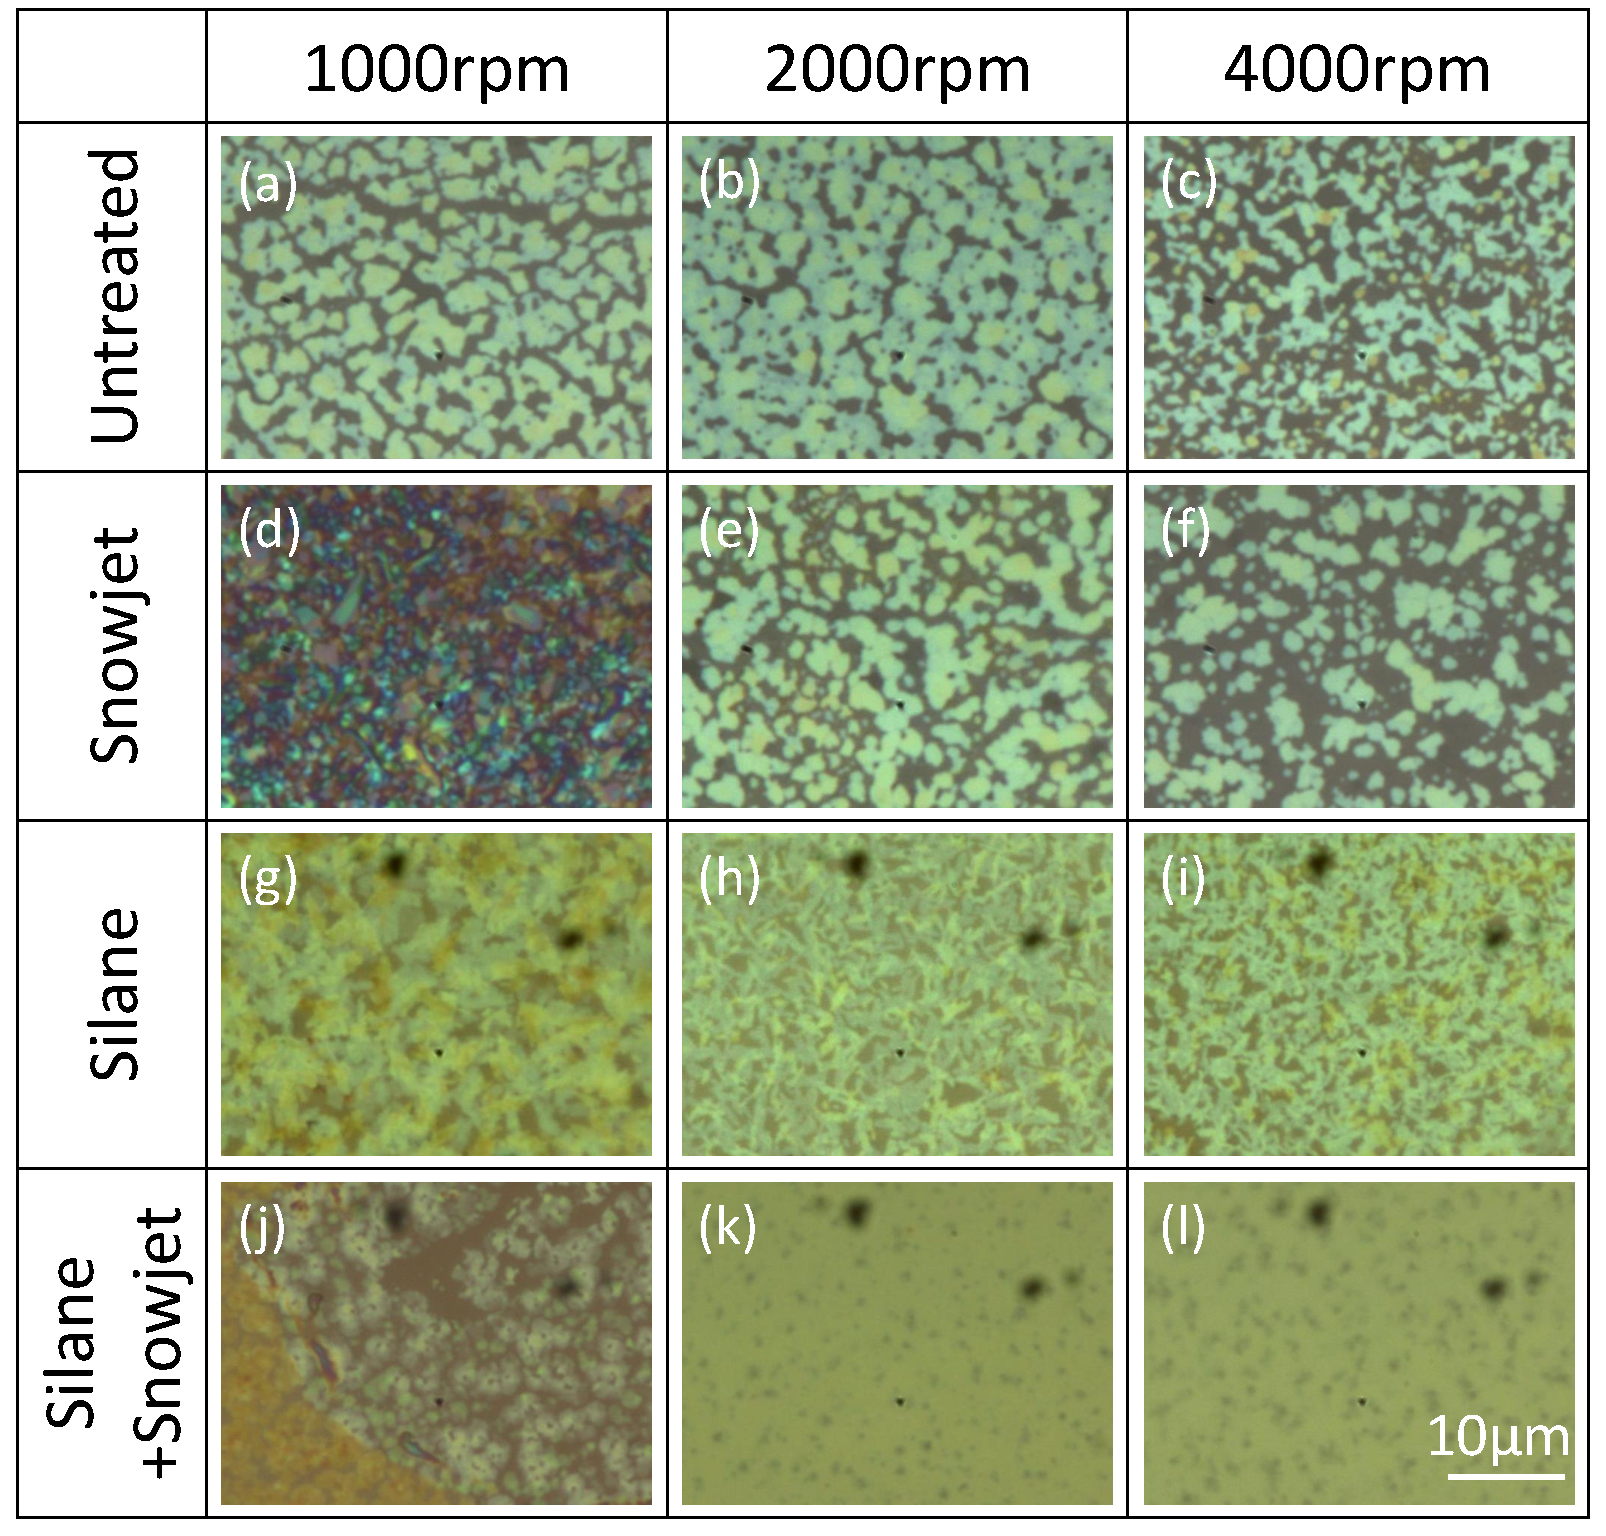
\includegraphics[width=0.8\textwidth]{Fig1}
\caption{BF images at 100$\times$ magnification of spin-coated C12PI films, with spin speed and substrate preparation as labelled. Note that (d) was formed while the substrate was heated, creating the non-uniform film observed.}
\label{4Fig1}
\end{figure}
BF images at 100$\times$ magnification of C12PI films made using a variety of spin coating conditions are shown in Fig.\,\ref{4Fig1}. Films showed significant dewetting without functionalisation of the substrate due to the hydrophobic nature of the organic molecule [Fig.\,\ref{4Fig1}(a-f)], and for this reason no films were formed on plasma etched substrates. Fig.\,\ref{4Fig1}(d) does not exhibit such dewetting as the substrate was heated before the application of the C12PI solution, thus the solvent evaporate before fluid could be removed by the centrifugal force, forming the extremely non-uniform film observed. Surface functionalisation due to APTES improved coverage of C12PI films due to stronger interactions between C12PI constituents and the amine groups. However a further snowjet cleaning steps removed any excess APTES left over from the silanisation step, removing some surface roughness and produced the most uniform C12PI samples.

\subsection{Spin speed}
\begin{figure}[ht]
\centering
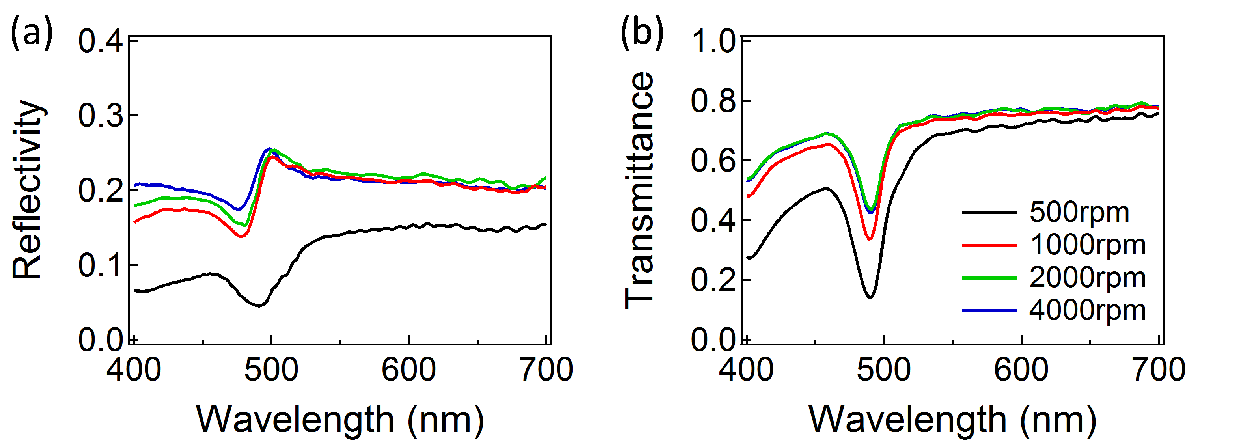
\includegraphics[width=\textwidth]{Fig2}
\caption{(a) Reflection and (b) transmission spectra for spin coated films on a silanised glass substrate at 5$\times$ magnification, collected over a $\sim20\,\mu$m diameter region.}
\label{4Fig2}
\end{figure}
Optical spectra of C12PI films created on silanised substrates collected over a region with diameter $\sim20\mu$\,m is shown in Fig.\,\ref{4Fig2}, and illustrates the general trends seen for all substrate preparations. The exction appears as a Fano resonance at $\approx500\,$nm in reflectivity spectra due to interference between its narrow narrow resonance and the continuum background, while a dip appears in the transmittance spectra. Although both phases of C12PI are observed for films on silanised substrates below 2000\,rpm, here we only consider areas exhibiting the high energy exciton. As spectra can be directly correlated to the images taken, we observe that the comparable morphologies of the films made above 1000\,rpm [Fig.\,\ref{4Fig1}(g-i)] does indeed produce similar spectra. The film made at 500\,rpm is rougher and less uniform in images, a fact reflected by the lowering of the overall reflectivity and Fano resonance shape. As C12PI is a multilayer system, the size of the exciton dip in transmission spectra can be used as a gauge of the film thickness, and here we observe that the film thickness decreases with spin speed as expected.

\subsection{Substrate preparation}
\begin{figure}[ht]
\centering
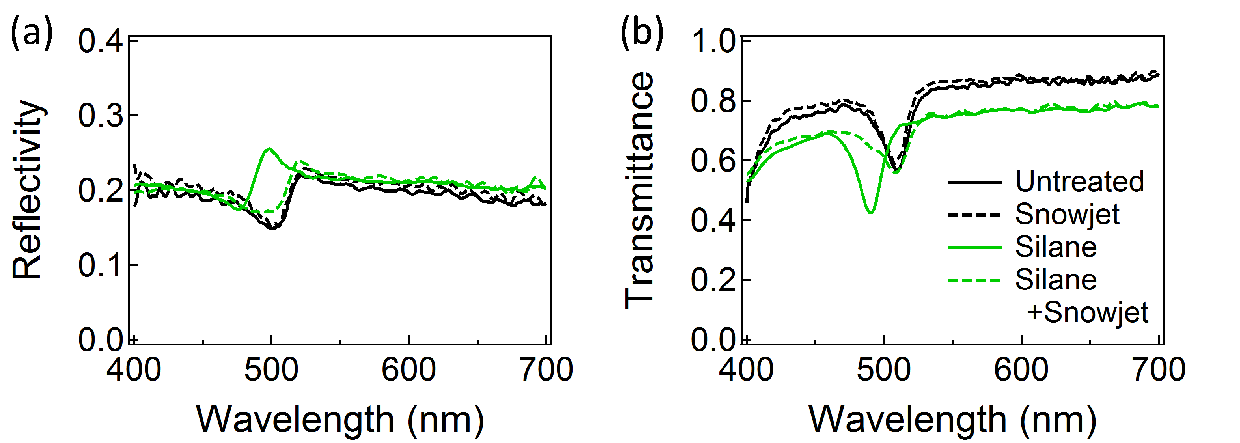
\includegraphics[width=\textwidth]{Fig3}
\caption{(a) Reflection and (b) transmission spectra for 4000\,rpm spin coated films using the labelled substrate preparation at 5$\times$ magnification, collected over a $\sim20\,\mu$m diameter region.}
\label{4Fig3}
\end{figure}
Optical spectra of 4000\,rpm C12PI films are shown in Fig.\,\ref{4Fig3}. The reflectivity spectra are very similar for all substrate preparations, with the exception of the silanised substrates where only the high energy phase was observed. This is most likely due to excess APTES molecules creating surface roughness, thus favouring the more crumpled C12PI phase. Removal of the excess silanes via snowjetting removes such roughness, so only the lower energy exciton is observed. Another difference is seen in the value of the transmittance at large wavelengths, where improved C12PI film coverage due to silane molecules leads to the lowering of the background transmittance.

\subsection{Sample degradation}
\begin{figure}[ht]
\centering
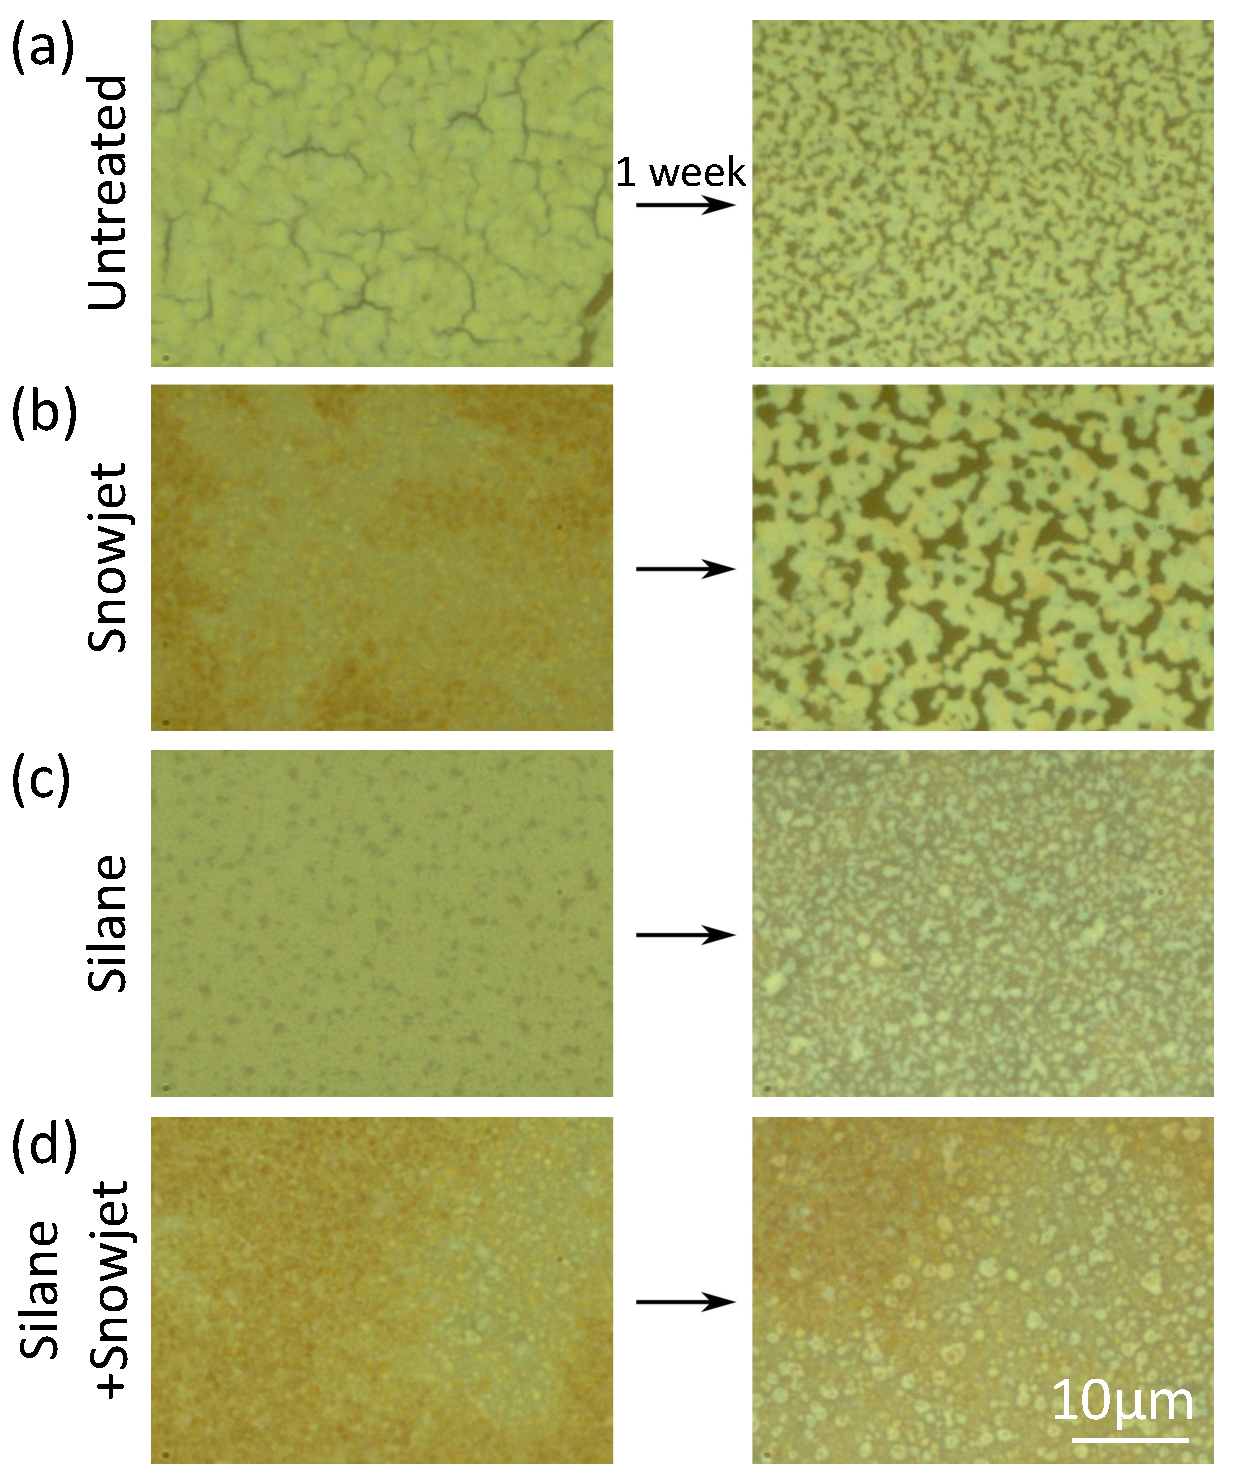
\includegraphics[width=0.8\textwidth]{Fig4}
\caption{Degradation of C12PI thin films shown in $100\times$ magnification BF images. Figures on the right were taken one week after those on the left, during which time samples were placed in standard conditions. All samples were produced at 2000\,rpm.}
\label{4Fig4}
\end{figure}
BF images at 100$\times$ magnification of 2000\,rpm films as-made (left) and after week under standard conditions (right) are shown in Fig.\,\ref{4Fig4}. All films showed signs of dewetting or diffusion during this time, indicating the importance of placing C$_n$PI films in low humidity atmospheres after formation, or capping with a polymer layer (e.\,g.\,Ref.\,\cite{Pradeesh2009}) to prevent sample degradation due to humidity in the atmosphere.

\section{CHPI thin films}
\begin{figure}[ht] 
\centering    
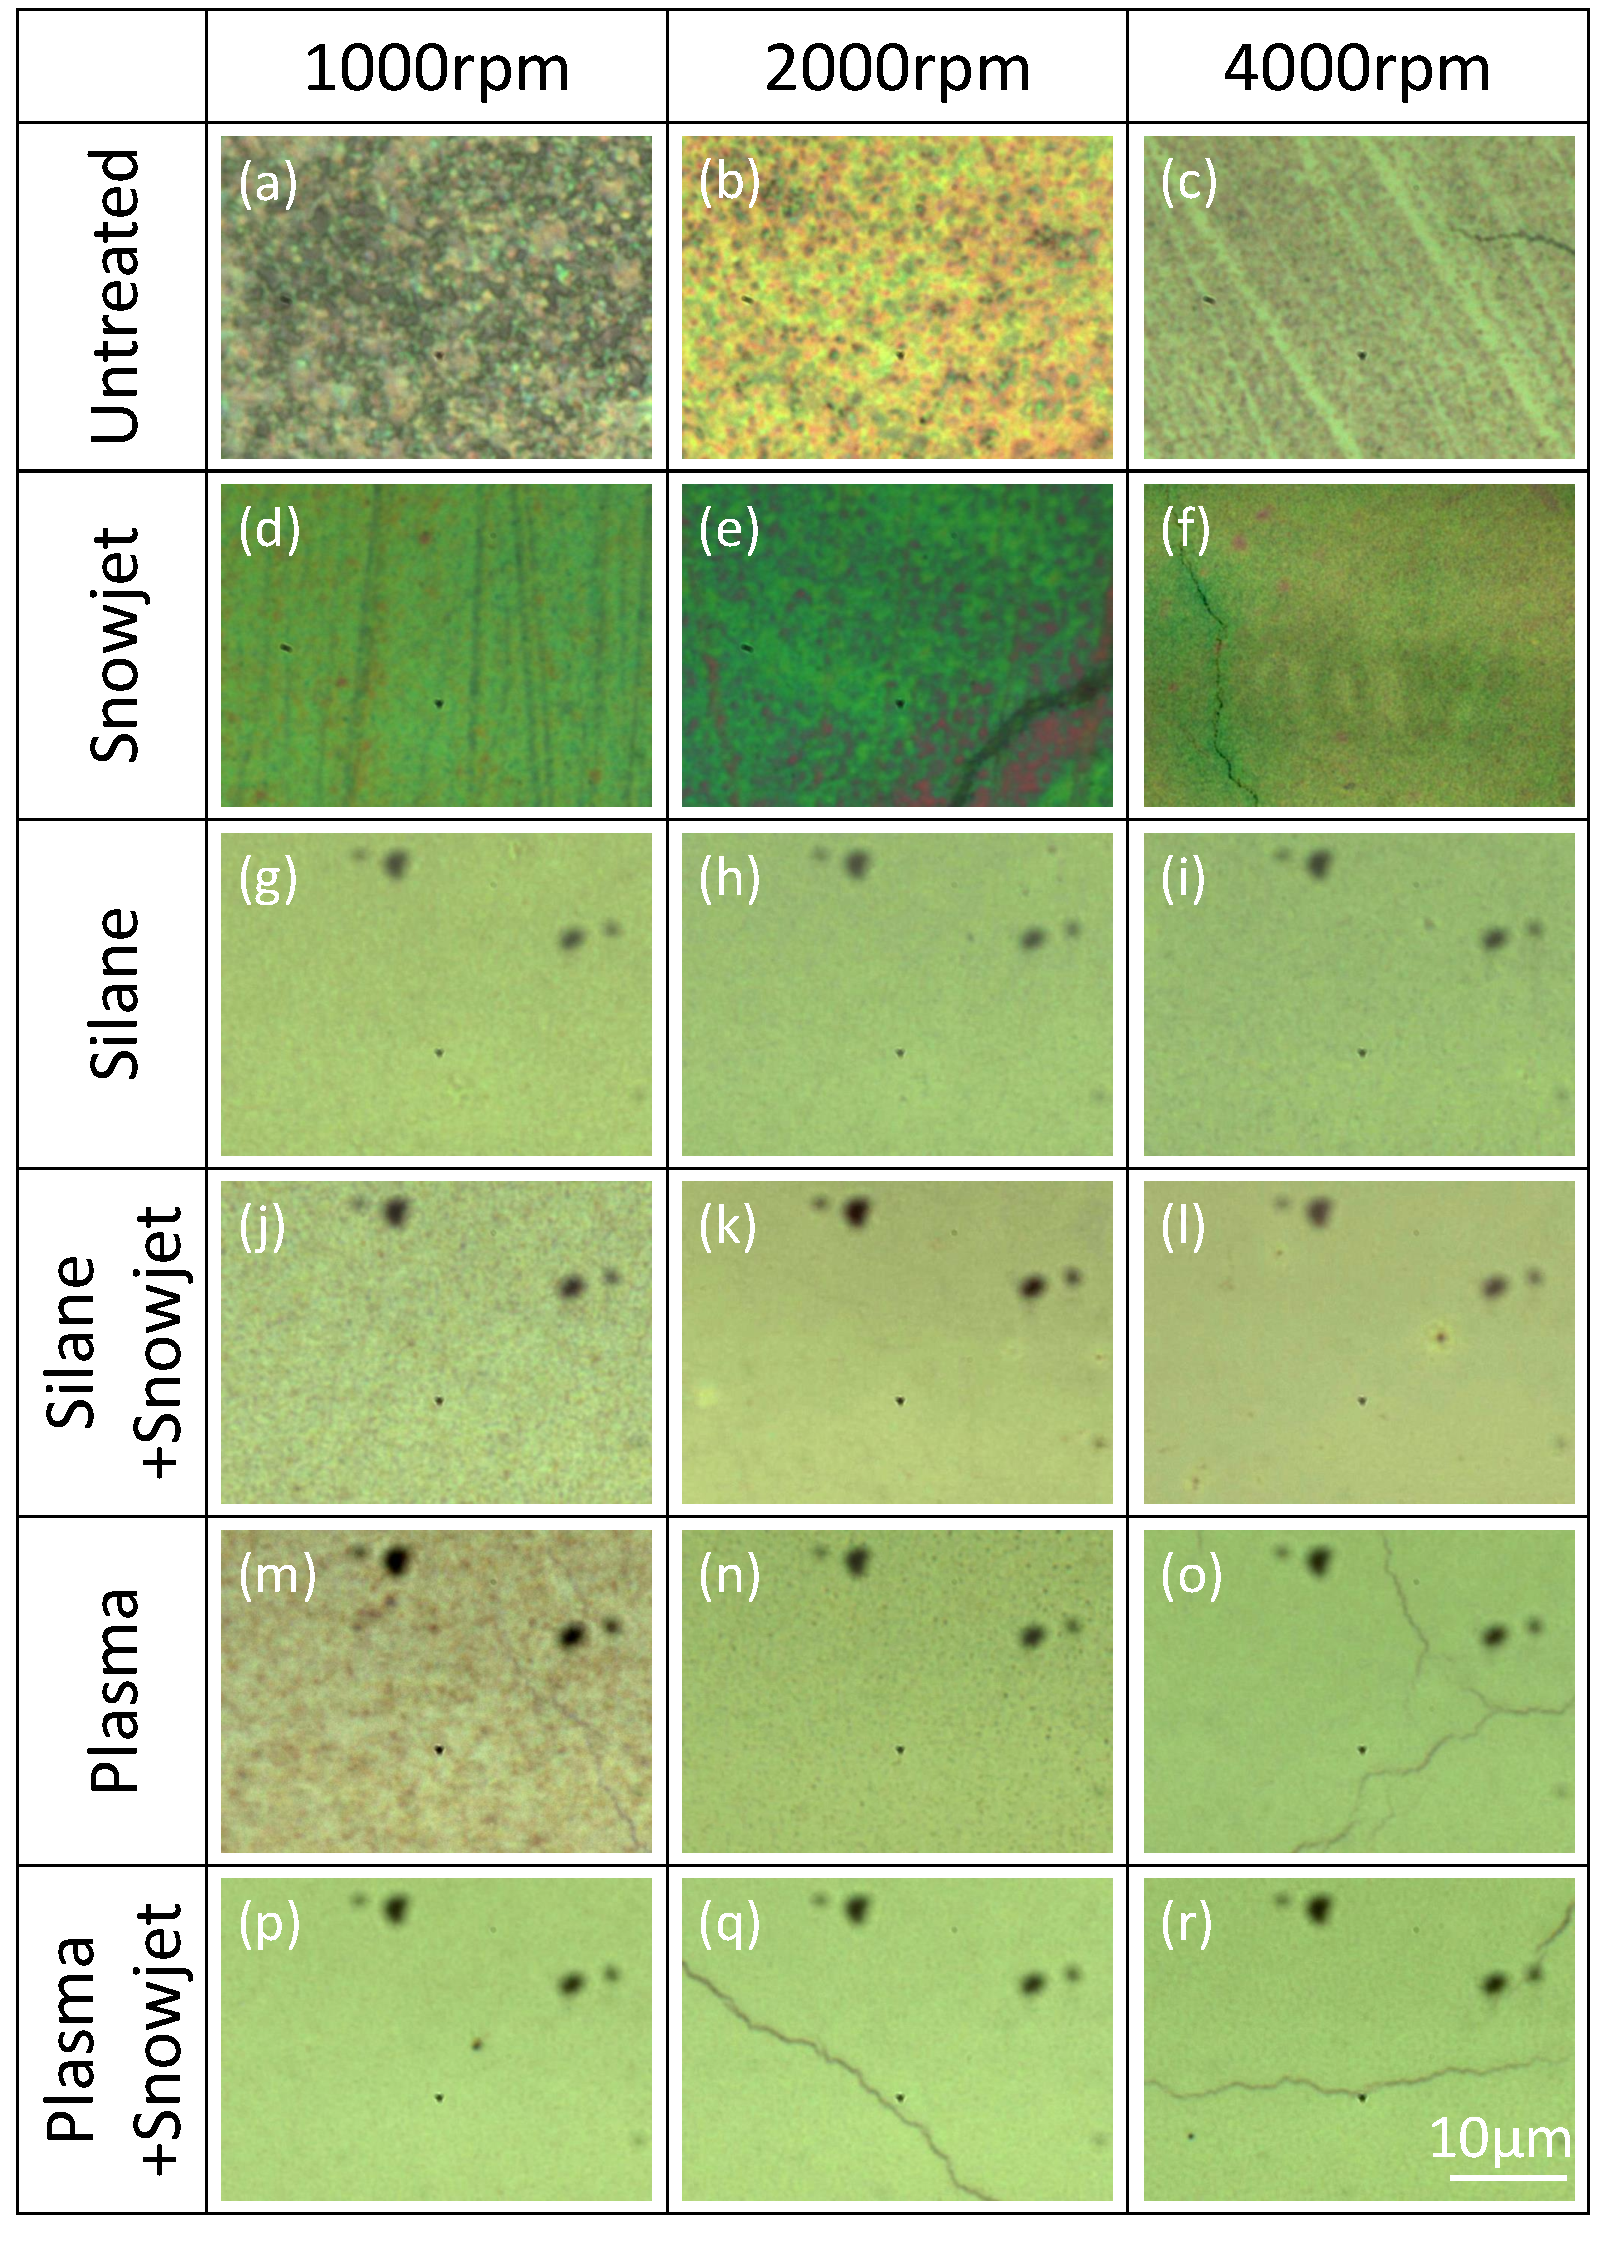
\includegraphics[width=0.8\textwidth]{Fig5}
\caption{BF images at 100$\times$ magnification of spin-coated CHPI films, with spin speed and substrate preparation as labelled.}
\label{4Fig5}
\end{figure}
BF images at 100$\times$ magnification of CHPI films made using a variety of spin coating conditions are shown in Fig.\,\ref{4Fig5}. No dewetting was observed with CHPI due to increased hydrophilicity of the organic molecule. Both snowketting and high spin speeds improved the uniformity of the samples. However, functionalisation of the substrate with APTES greatly improved the film quality, and in this case the improvement with spin speed was minimal. A similar effect was seen in plasma etched substrates.

\subsection{Spin speed}
\begin{figure}[] 
\centering    
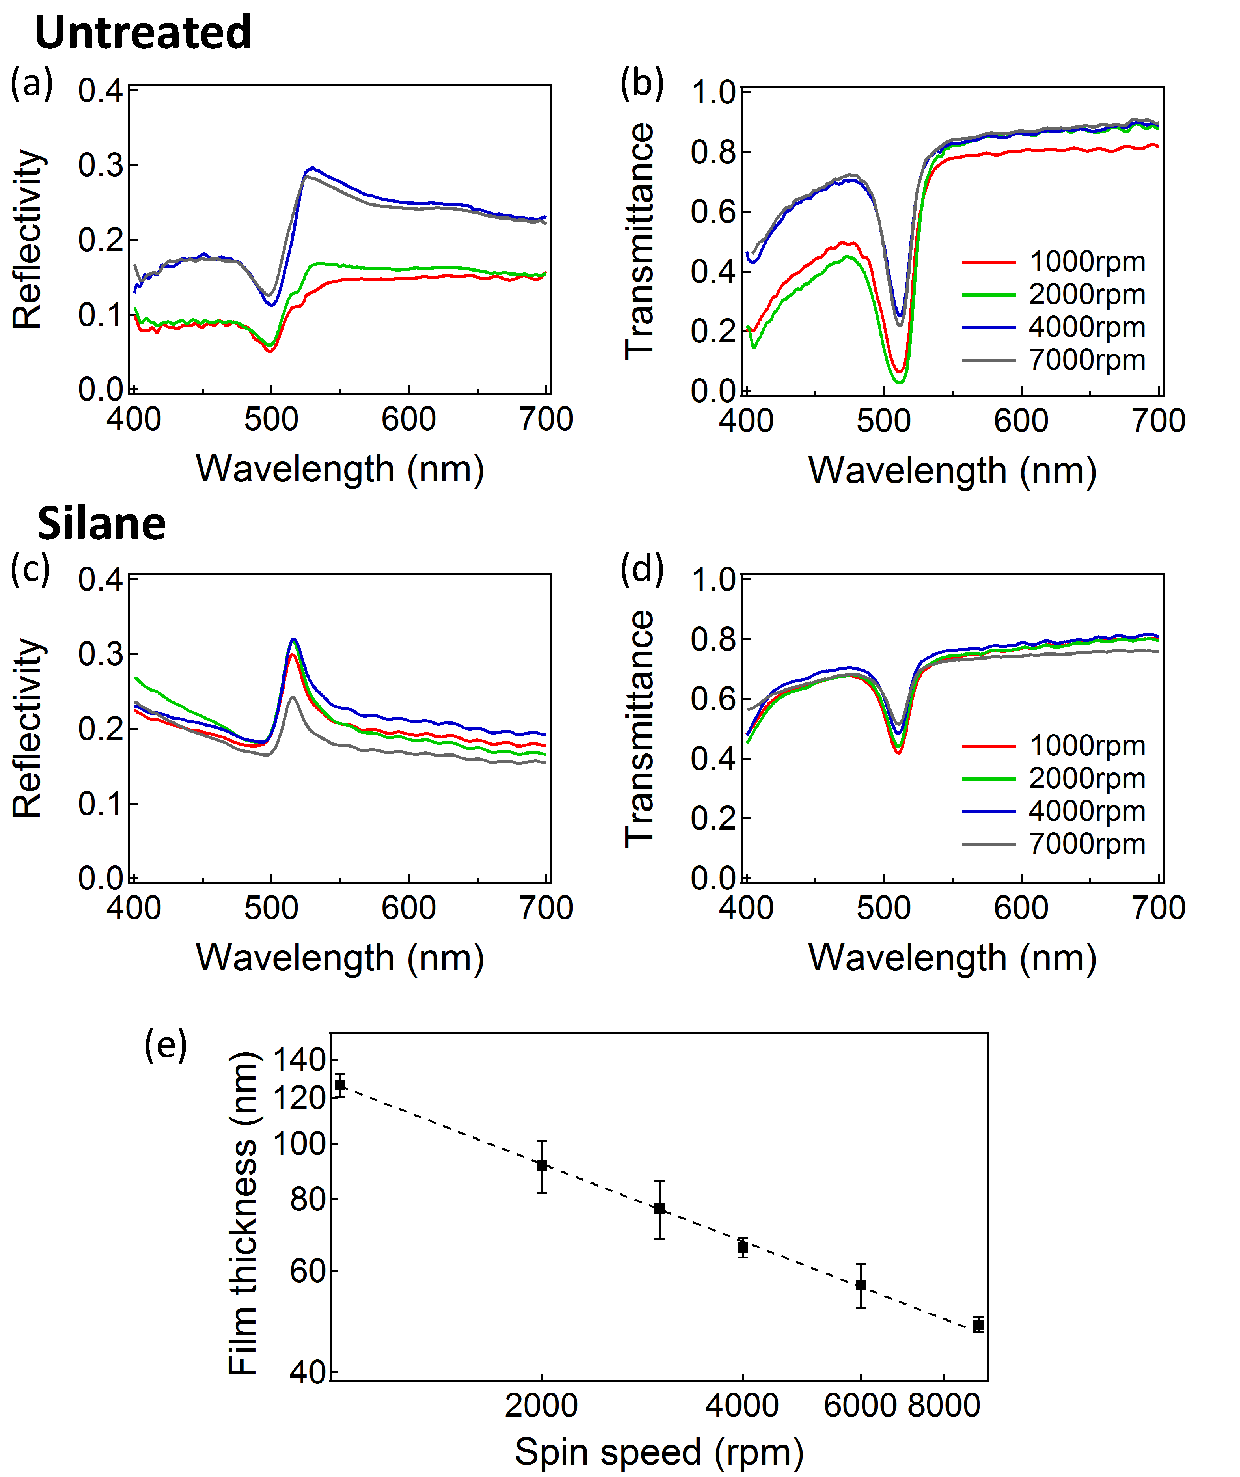
\includegraphics[width=\textwidth]{Fig6}
\caption{Reflection and transmission spectra collected at 5$\times$ magnification over a $\sim20\,\mu$m diameter region, on films prepared on (a,b) untreated and (c,d) silanised substrates. (e) Effect of spin speed on CHPI film thickness prepared on untreated substrates for 30\,mg/ml solutions. The dashed lines indicate fit to the form $ax^b$, with $b=-0.449\pm0.009$.}
\label{4Fig6}
\end{figure}
Optical spectra of CHPI films created on silanised substrates collected over a region with diameter $\sim20\mu$\,m is shown in Fig.\,\ref{4Fig6} for untreated and silanised substrates. For untreated substrates, a change in the shape of recorded spectra between 1000 and 2000\,rpm indicate a change in morphology: at low spin speeds a lower reflectivity indicate increase film roughness, and the appearance of a second higher energy exciton can be seen, leading to an increase in the linewidth of the transmission dip. Such extra resonances have been observed for thick perovskite films, and is attributed to stacking faults, strain and structural misalignment in the structure \cite{VijayaPrakash2009}. In contrast, the spectra for silanised substrates are very similar, as expected from their BF images [Fig.\,\ref{4Fig5}(g-i)]. Although the amplitude of the exciton features change due to film thickness, the similarity in the spectra indicate similar film morphologies. Film thickness measurements for around 10 films made using untreated substrates [Fig.\,\ref{4Fig6}(e)] show an $\omega^{-0.45}$ dependence to the film thickness, similar to the $\omega^{-0.5}$ relationship predicted by theory. 

\subsection{Substrate preparation}
\begin{figure}[] 
\centering    
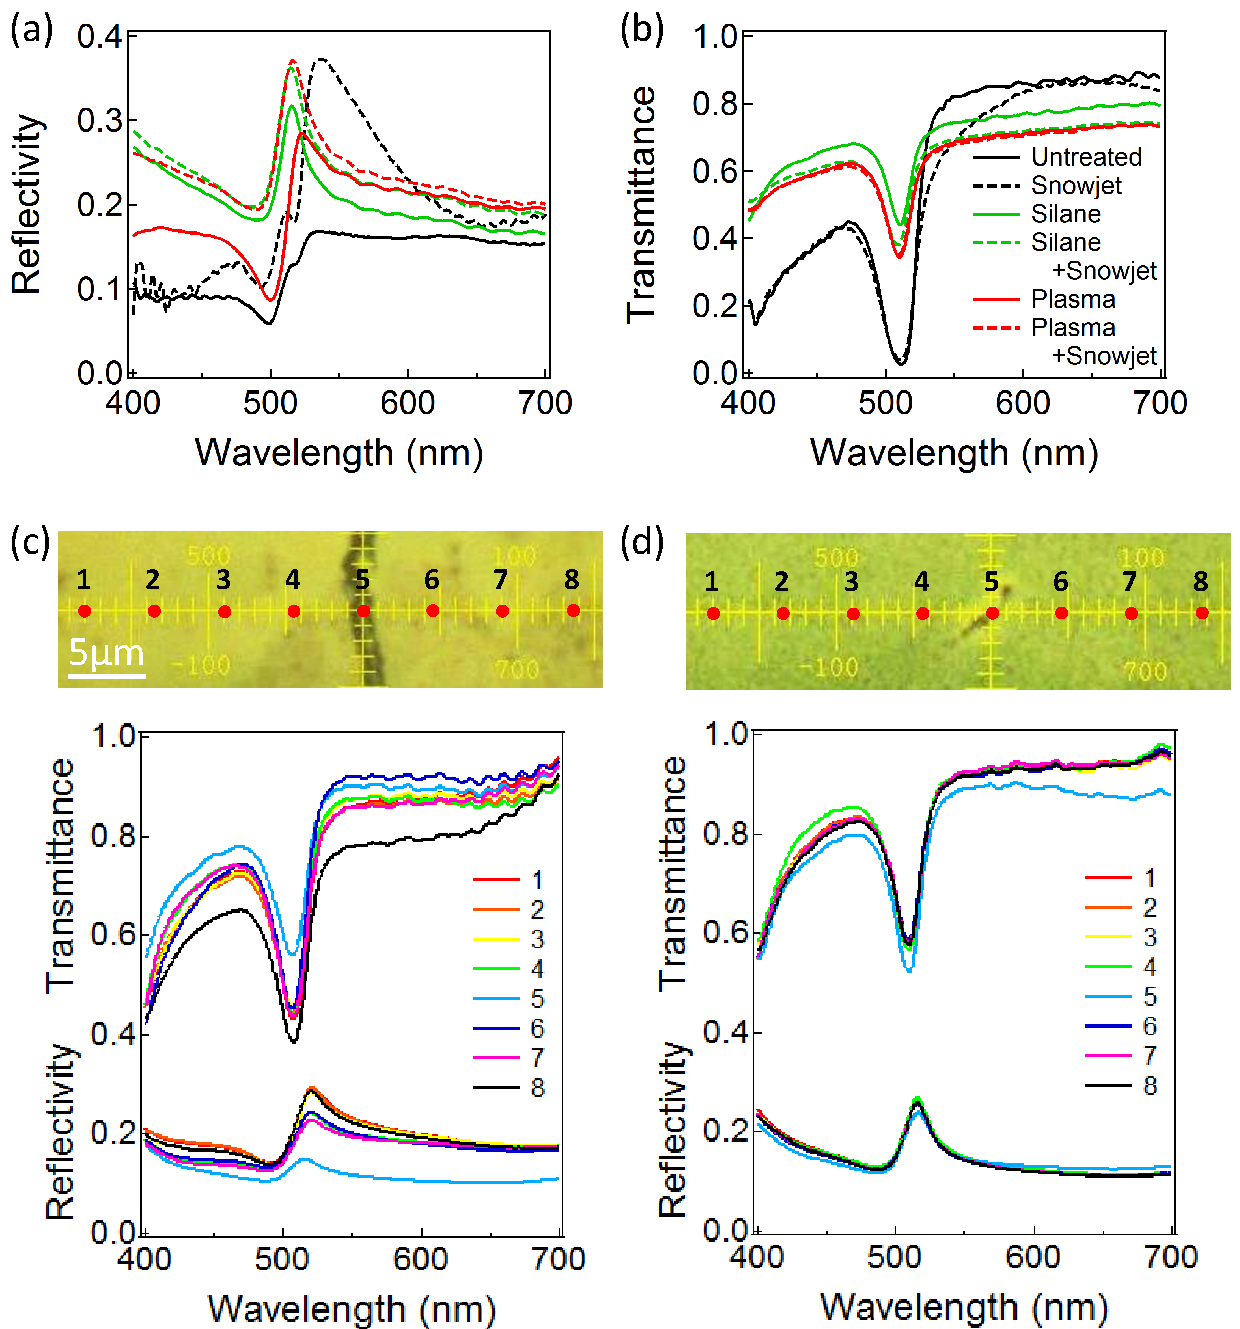
\includegraphics[width=\textwidth]{Fig7}
\caption{Reflection and transmission spectra collected at 5$\times$ magnification over a $\sim20\,\mu$m diameter region, on 2000\,rpm films created using the labelled substrate preparation. Reflection and transmission spectra collected at 100$\times$ magnification over a $\sim1\,\mu$m diameter region, on 4000rpm films prepared on (c) untreated and (d) silanised and snowjetted substrate at the positions indicated.}
\label{4Fig7}
\end{figure}
Optical spectra of 4200\,rpm CHPI films are shown in Fig.\,\ref{4Fig7}. The appearance of a second exciton due to structural misalignment is seen in both untreated and snowjetted films. However as indicated by BF images [Fig.\,\ref{4Fig5}(h,k,n,q)], the spectra and morphologies of films using other substrate preparations are very similar, and the uniformity is greatly improved by functionalisation of the substrate via silanisation or plasma etching. To test the uniformity, spectra of different regions on a 4000\,rpm film made on untreated [Fig.\,\ref{4Fig7}(c)] and silanised and snowjetted [Fig.\,\ref{4Fig7}(d)] substrates are taken, and the near-identical spectra for all areas tested on the functionalised substrate is proof of the uniformity observed in BF images.

\subsection{Humidity}
\begin{figure}[] 
\centering    
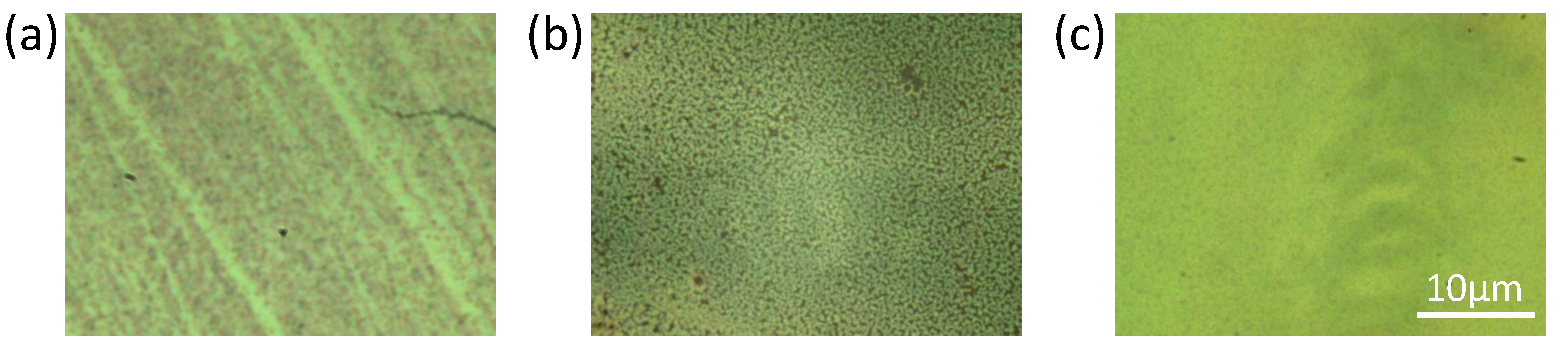
\includegraphics[width=\textwidth]{Fig8}
\caption{BF images at 100$\times$ magnification for 4000\,rpm films made on untreated substrates in (a) low, (b) high and (c) dehydrated atmospheres in the spin coater.}
\label{4Fig8}
\end{figure}
Hydrogen bonding between the organic and inorganic constituents holds the structure together, and as such the self-assembly can be disrupted by water in the atmosphere. Fig.\,\ref{4Fig8}(a) shows the morphology of a 4000\,rpm CHPI film on an untreated substrate at 100$\times$ magnification in a low humidity atmosphere (October), and a continuous film is formed as expected. However using the same conditions in a high humidity atmosphere leads to dewetting of the film [Fig.\,\ref{4Fig8}(b)] despite the more hydrophilic organic group. Therefore the level of humidity in the spin coater is very important to film formation, and as much water should be removed from the environment as possible. In order to achieve this, the dehydration agent \ce{CaCl2} is placed inside the spin coater for roughly an hour before film production, and the spin coater pumped with \ce{N2} just before use. The resulting film [Fig.\,\ref{4Fig8}(c)] is extremely uniform without modification of substrate functionalisation, and produces similar films under all conditions.

\section{Conclusions}
Thin films of PbI perovskites with thickness $\sim10$s\,nm are produced reliably using spin coating. The morphology of such films depends on the organic molecule within the perovskite structure, and dewetted films are produced for more hydrophobic moeities. However film coverage and uniformity can be improved by functionalisation of the substrate surface using techniques such as silanisation. Higher spin speeds can also be used to produce more uniform films. The film thickness is controlled by the spin speed or initial solution concentration. Formation of the perovskite structure can also be disrupted by water in the atmosphere, and a dehydration agent should be placed in the spin coater to produce a controllably low humidity environments. The simplicity and adaptability of spin coating allows PbI perovskite thin films to be deposited onto nanostructured substrates.